\chapter{Click-through Rate (CTR) Prediction}
\label{chapterlabel2}

In this chapter, we describe the dataset that we use for CTR prediction and then introduce some preprocessing and feature engineering techniques. Three advanced and practical models are included. They are Bayesian Online Probit Regression (BOPR), Follow the Regularized Leader (FTRL) and Field-aware Factorization Machine (FFM) respectively. The following Figure~\ref{fig:flowchart} is the workflow of the CTR estimation.

\begin{figure}[h]
\centering
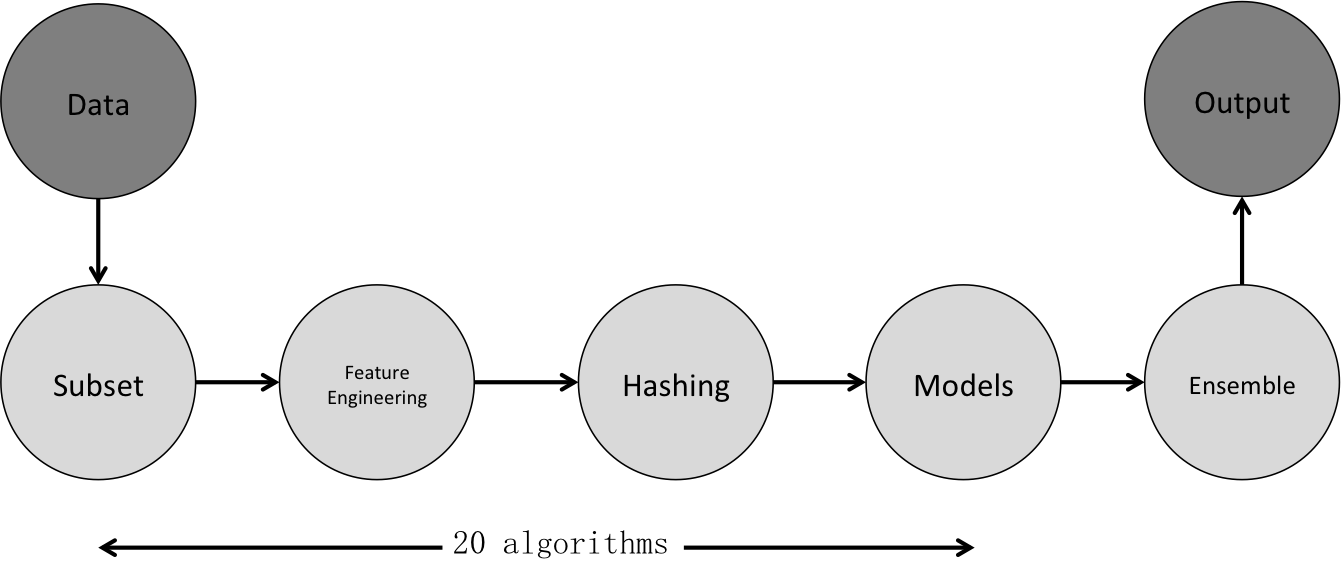
\includegraphics[width=0.9\textwidth]{flowchart.png}
\caption{The work flow chart of CTR estimation procedure}
\label{fig:flowchart}
\end{figure}

\section{Origins of Data Features}
RTB is a well-studied problem in online advertising as most of researches only limit to keyword auction in the context of sponsored search. It is fundamentally different and based on a second price auction \cite{williamvickrey1961}, which has recently emerged as a new display advertising paradigm \cite{zhang2015statistical, zhang2014real, Zhang:2014:ORB:2623330.2623633}. Unlike traditional sponsored search or contextual advertising, where an advertiser presets a bid price for each keyword chosen for their campaigns, advertisers bid for each given impression in RTB. The process takes less than 100ms time frame. Besides, RTB is a type of programmatic buying, which means automated the buying, placement and optimization of ad inventory. Comparing to RTB, some publishers sell their inventory in advance with a fixed price. The bidding price is based on Key Performance Indicator (KPI) like CTR. The whole process is an auction game \cite{zhang2014real}.

The payment and revenue formally consists of three elements: Page View (PV), Click-through Rate (CTR) and Cost per Click (CPC). CTR will be used for the valuation of ads for advertisers and revenue model of ads for publishers. As a consequence, the management of CTR is absolutely crucial to advertising and its corresponding business value.

In this project, we use the RTB data from iPinYou as our training and test dataset. The dataset includes 26 features shown in Table~\ref{tab:features}.

\begin{table}[h]
\caption{The log data format of iPinYou dataset.}
\label{tab:features}
\begin{center}
\begin{tabular}{ l l l } 
\hline
Col & Description & Example \\
\hline
1 & Bid ID & 0150008...3g4fa5621 \\ 
2 & Timestamp & 20129220001004721 \\ 
3 & Log type & 1 \\ 
4 & iPinYou ID & 48598757396839735 \\
5 & User-Agent & windows-chrome \\
6 & IP & 117.86.123.* \\
7 & Region & 16 \\
8 & City & 11 \\
9 & Ad exchange & 1 \\
10 & Domain & trqRTvNNQIj7gspy \\
11 & URL & bebefa5efe83...45e7c50b \\
12 & Anonymous URL ID & null \\
13 & Ad slot ID & 3582857028 \\
14 & Ad slot width & 336 \\
15 & Ad slot height & 280 \\
16 & Ad slot visibility & 2 \\
17 & Ad slot format & 0 \\
18 & Ad slot floor price & 5 \\
19 & Creative ID & 778d3...16d68ad923a1 \\
20 & Bidding price & 300 \\
21 & Paying price & 118 \\
22 & Key page URL & bebefa5ef...45e7c5085b \\
23 & Advertiser ID & 1458 \\
24 & User Tags & 13042,10057,10006 \\
25 & Weekday & 6 \\
26 & Hour & 0 \\
\hline
\end{tabular}
\end{center}
\end {table}

In general,  the auction and ad features (all columns except 3, 20 and 21) are categorical data that are sent to bidding engine to make a bid response. The auction winning price (column 21) is a numerical integer. If the highest price is larger this, the Demand side platform (DSP) will win this impression. The user feedback (click and conversion) on this ad impression (column 3) is the target of the dataset. As we mainly focus on the prediction of CTR, the label is a binary number. The clickability of the ad depends on the type of ad and user. It is not relevant to the bidding aspect. Thus, the data we use to estimate CTR model is a categorical input. Table~\ref{tab:Advertiser} shows the summary of advertiser diversity. The advertiser from different field has various bidding behavior.

\begin{table}[H]
\caption{Advertiser fields and statistics}
\label{tab:Advertiser}
\begin{center}
\begin{tabular}{ l l l l l l l l l } 
\hline
Advertiser ID & Season & Period & Bids & Impressions & Clicks & CTR \\
\hline
1458 & 2 & 6-12 Jun & 14,701,496 & 3,083,056 & 2,454 & 0.080\% \\
2259 & 3 & 19-22 Oct & 2,987,731 & 835,556 & 280 & 0.034\% \\
2261 & 3 & 24-27 Oct & 2,159,708 & 687,617 & 207 & 0.030\% \\
2821 & 3 & 21-23 Oct & 5,292,053 & 1,322,561 & 843 & 0.064\% \\
2997 & 3 & 23-26 Oct & 1,017,927 & 312,437 & 1,386 & 0.444\% \\
3358 & 2 & 6-12 Jun & 3,751,016 & 1,742,104 & 1,358 & 0.078\% \\
3386 & 2 & 6-12 Jun & 14,091,931 & 2,847,802 & 2,076 & 0.073\% \\
3427 & 2 & 6-12 Jun & 14,032,619 & 2,593,765 & 1,926 & 0.074\% \\
3476 & 2 & 6-12 Jun & 6,712,268 & 1,970,360 & 1,027 & 0.052\% \\
Total & 2,3 & - & 64,746,749 & 15,395,258 & 11,557 & 0.075\% \\
\hline
\end{tabular}
\end{center}
\end {table}

We display basic statistics based on user feedback on advertisers of training dataset. Specifically, they are the mean value with the standard error of CTR against some features, such as weekday, hour, user agent, region, city, slot size and ad exchange, etc. From Figure~\ref{fig:advertiserstatistics}, we can see that different advertisers have various users' preference, which results in different impact on CTR.

\begin{figure}[htbp]

\begin{subfigure}{0.5\textwidth}
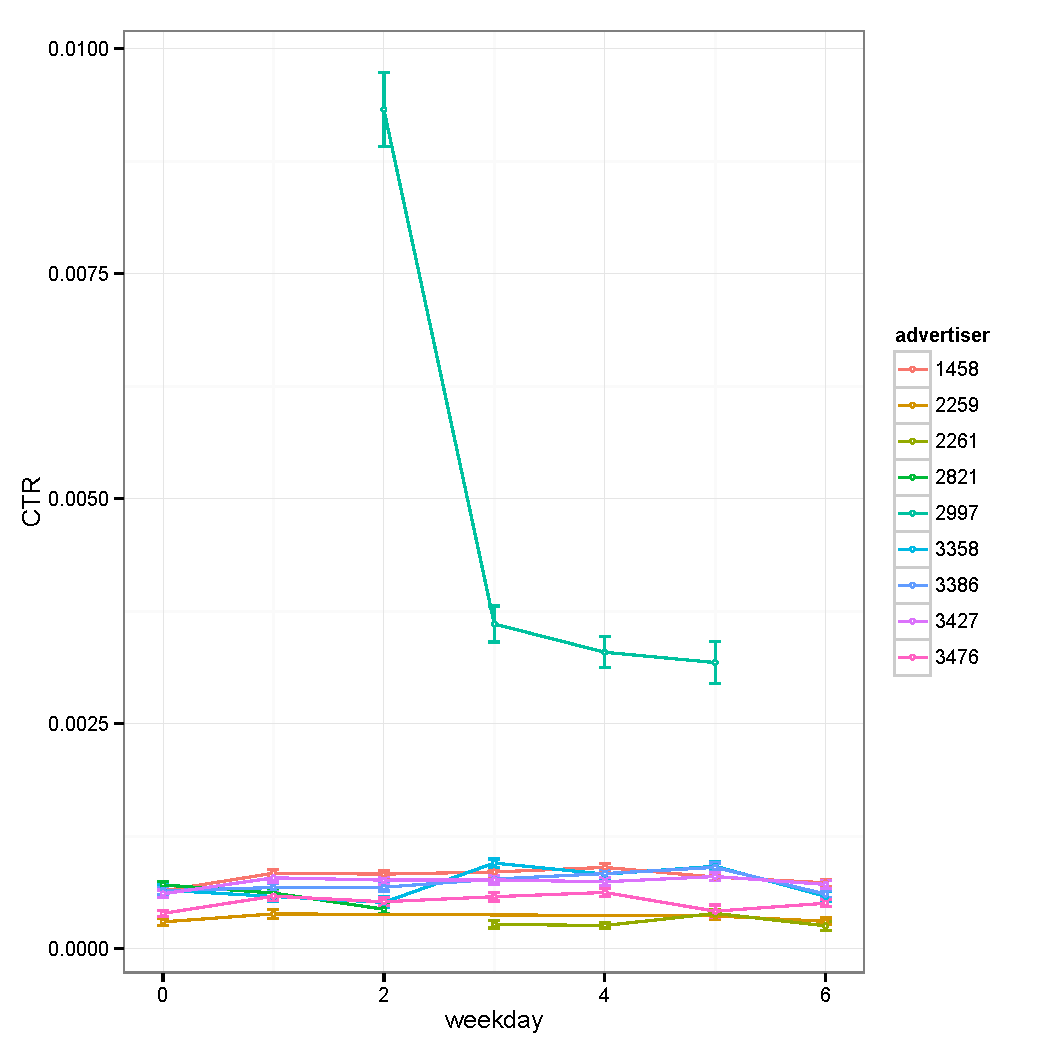
\includegraphics[width=0.9\linewidth, height=5cm]{weekday.pdf}
\caption{Weekday}
\label{fig:weekday}
\end{subfigure}
\begin{subfigure}{0.5\textwidth}
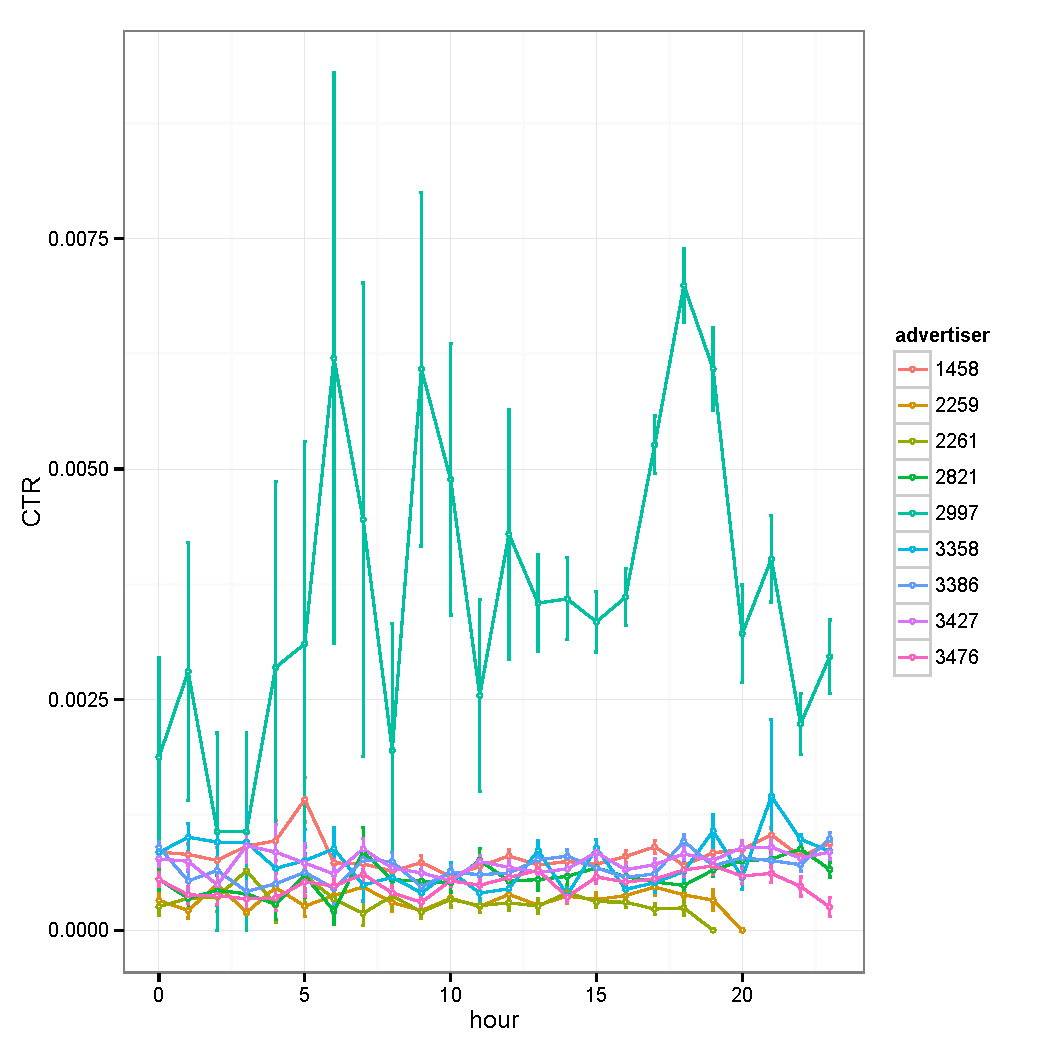
\includegraphics[width=0.9\linewidth, height=5cm]{hour.pdf}
\caption{Hour}
\label{fig:hour}
\end{subfigure}
\begin{subfigure}{0.5\textwidth}
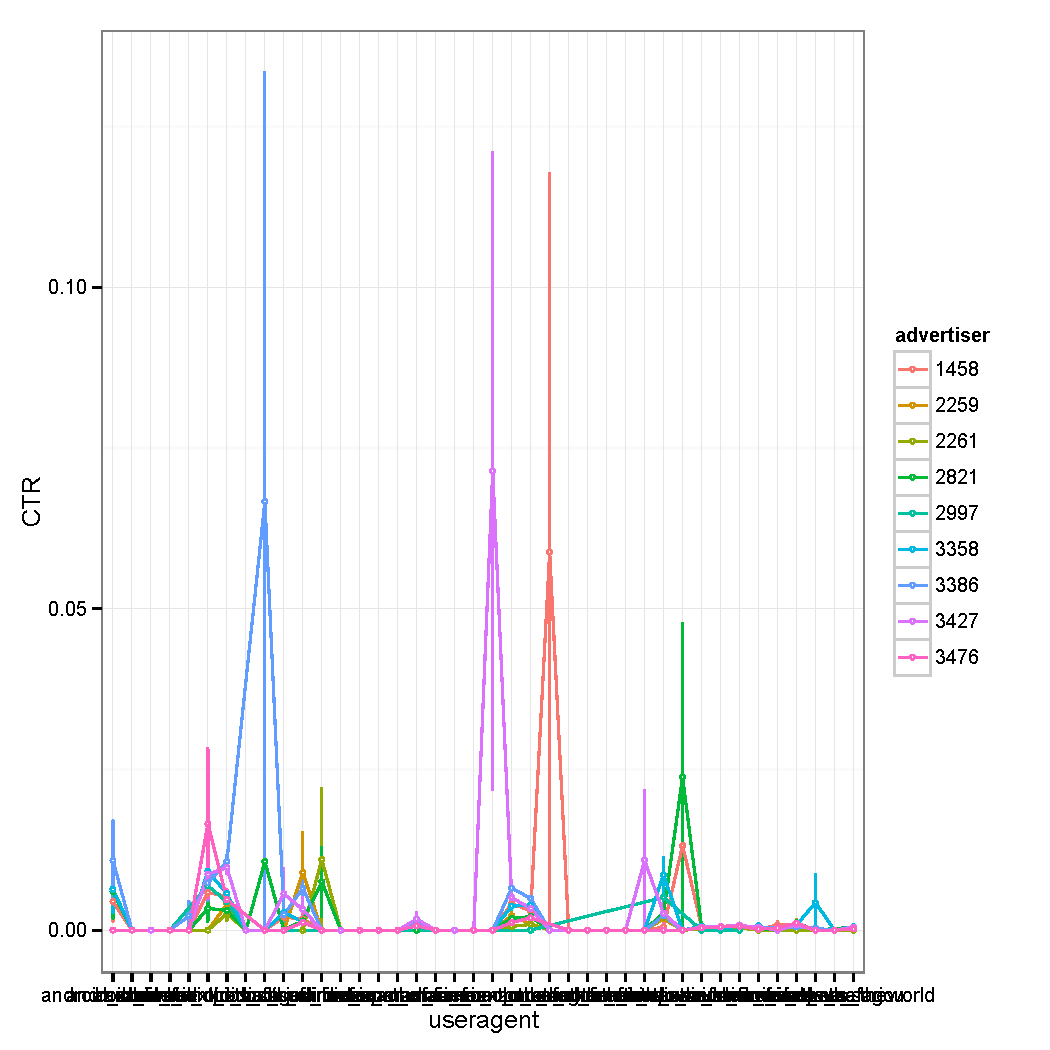
\includegraphics[width=0.9\linewidth, height=5cm]{useragent.pdf}
\caption{Useragent}
\label{fig:useragent}
\end{subfigure}
\begin{subfigure}{0.5\textwidth}
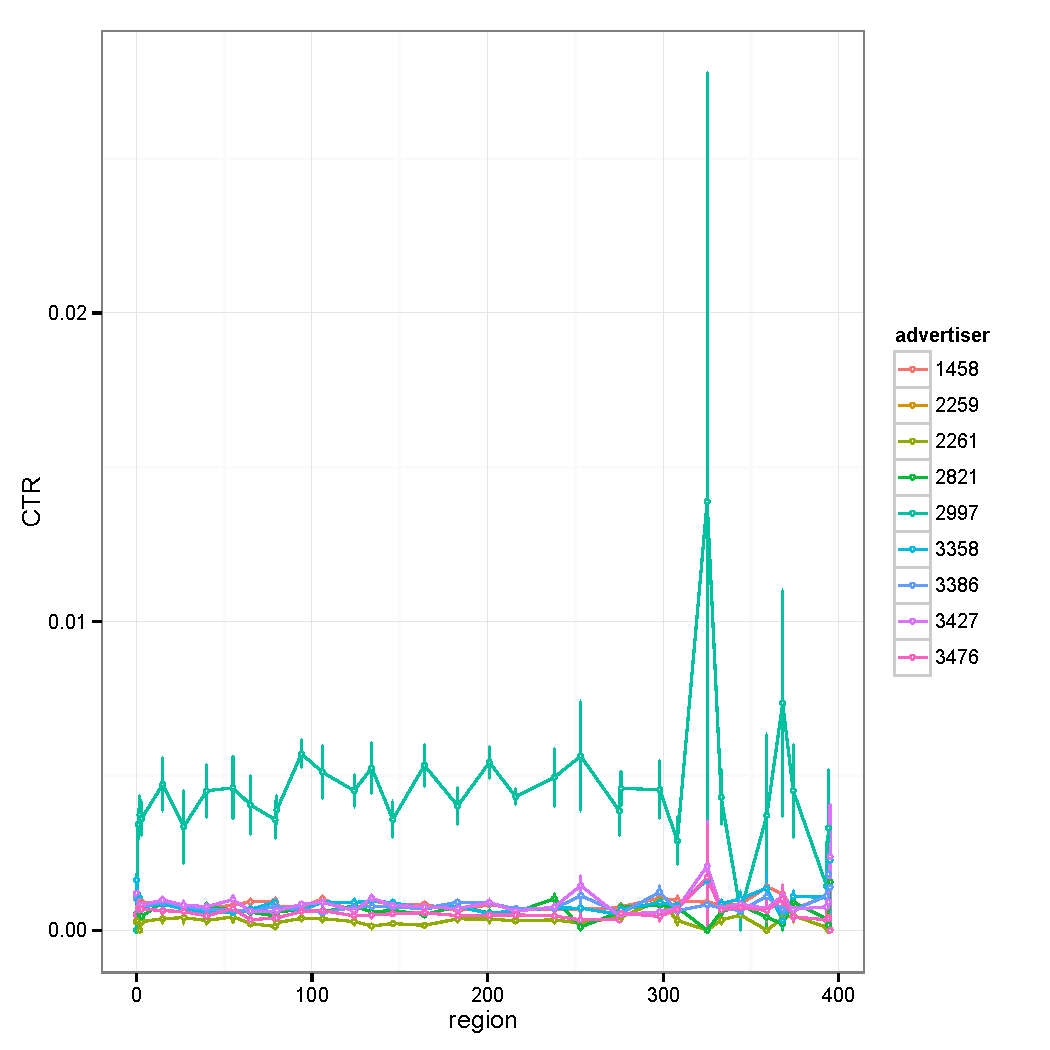
\includegraphics[width=0.9\linewidth, height=5cm]{region.pdf}
\caption{Region}
\label{fig:region}
\end{subfigure}
\begin{subfigure}{0.5\textwidth}
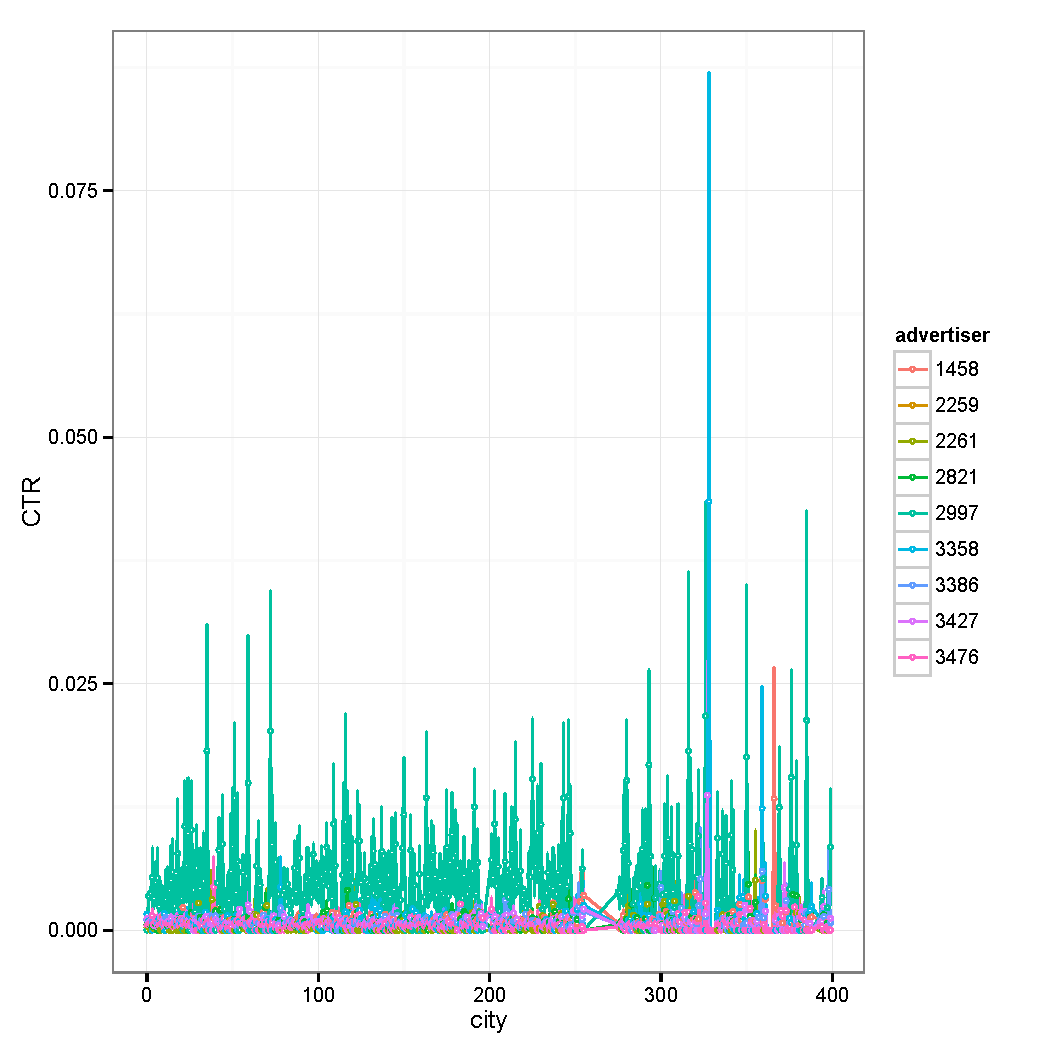
\includegraphics[width=0.9\linewidth, height=5cm]{city.pdf}
\caption{City}
\label{fig:city}
\end{subfigure}
\begin{subfigure}{0.5\textwidth}
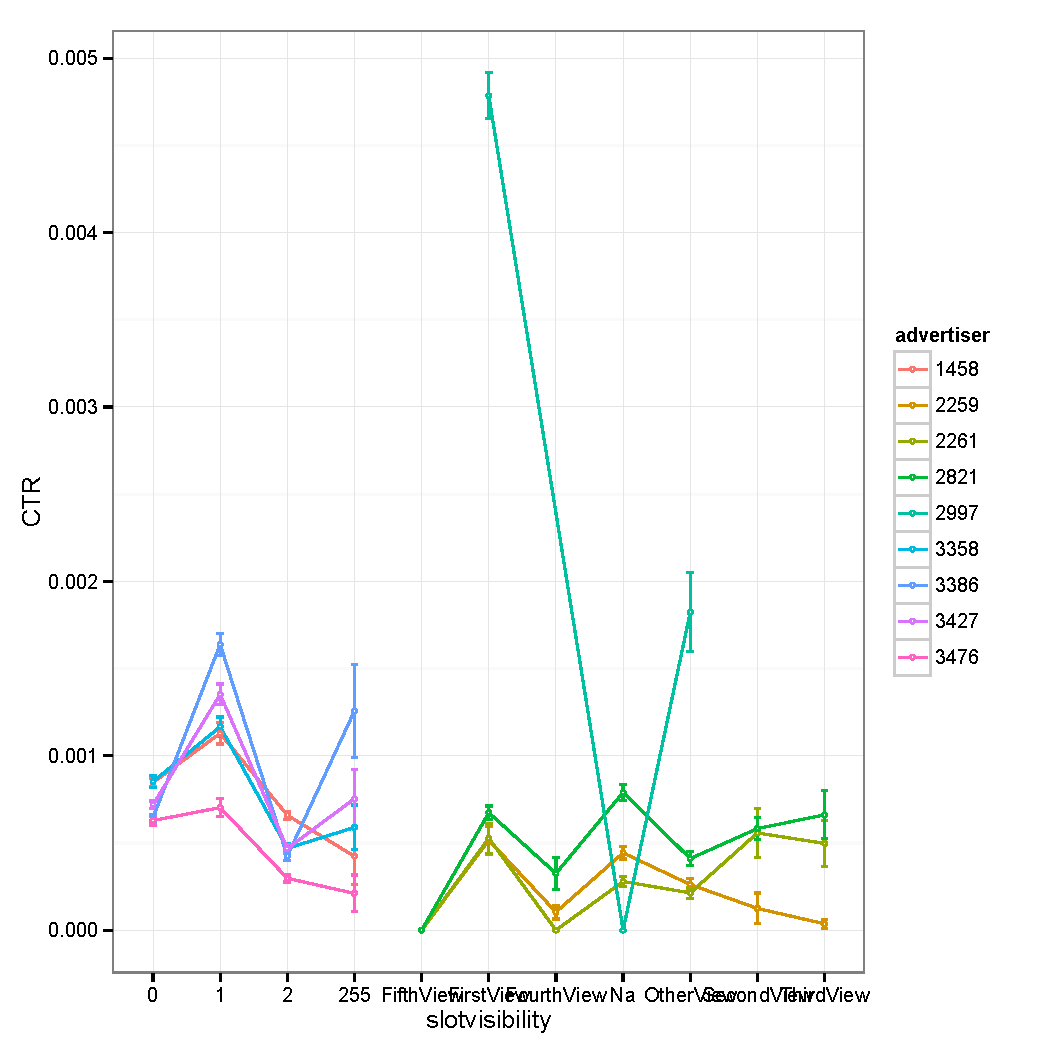
\includegraphics[width=0.9\linewidth, height=5cm]{visibility.pdf}
\caption{Visibility}
\label{fig:visibility}
\end{subfigure}
\begin{subfigure}{0.5\textwidth}
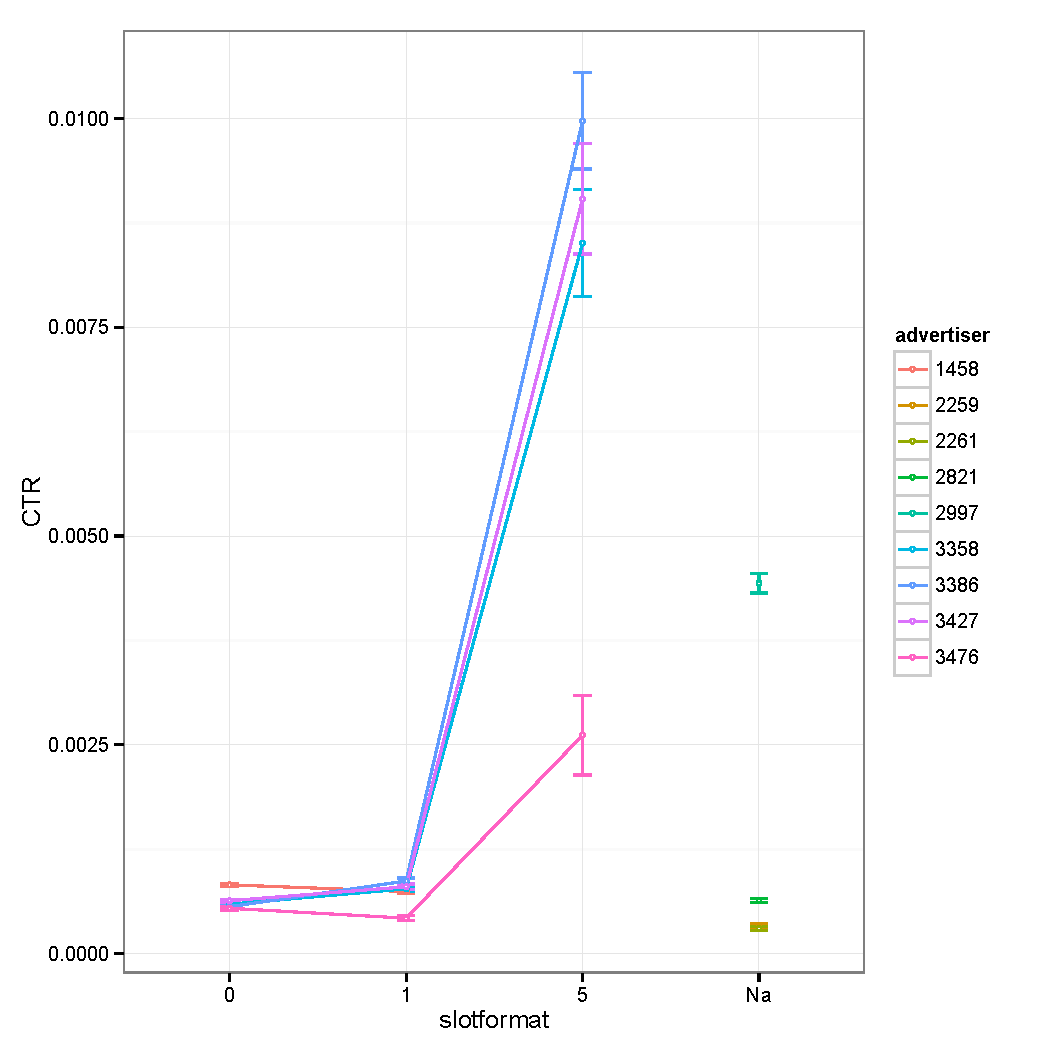
\includegraphics[width=0.9\linewidth, height=5cm]{format.pdf}
\caption{Format}
\label{fig:format}
\end{subfigure}
 \begin{subfigure}{0.5\textwidth}
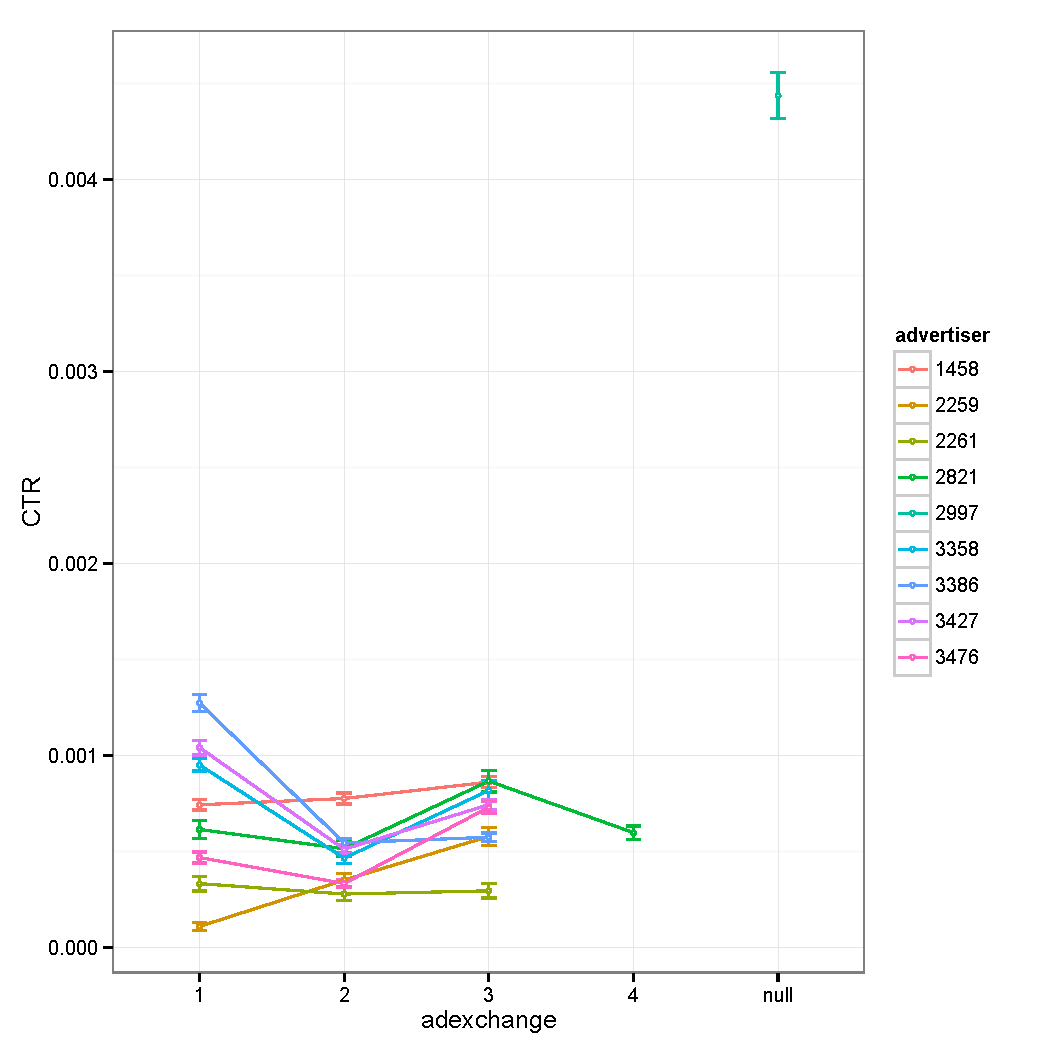
\includegraphics[width=0.9\linewidth, height=5cm]{exchange.pdf}
\caption{Exchange}
\label{fig:exchange}
\end{subfigure}

\caption{CTR distribution against different features of all advertisers}
\label{fig:advertiserstatistics}
\end{figure}

\section{Preprocessing and Feature Engineering}

Except the original categorical features, we can use tree model like \emph{Random Forest} (RF) and \emph{Gradient Boosting Descent Tree} (GBDT) to generate new features. Adding high order combination features is a variant and trick to better predicting performance. This approach is proposed by Facebook \cite{xinranhejunfengpanetc2014}. The details of RF and GBDT can refer to \cite{jeromeh.friedman1999}. A concrete example of implementation is shown in Figure~\ref{fig:GBDT}. Assume that we have already trained GBDT with 3 trees with depth 2. We feed an impression $\mathbf{x}$ into these trees. The first tree thinks $\mathbf{x}$ belong to node 4, the second node 7, and the third node 6. Then we generate a new feature 1:4 2:7 3:6 for this impression.

\begin{figure}[htbp]
\centering
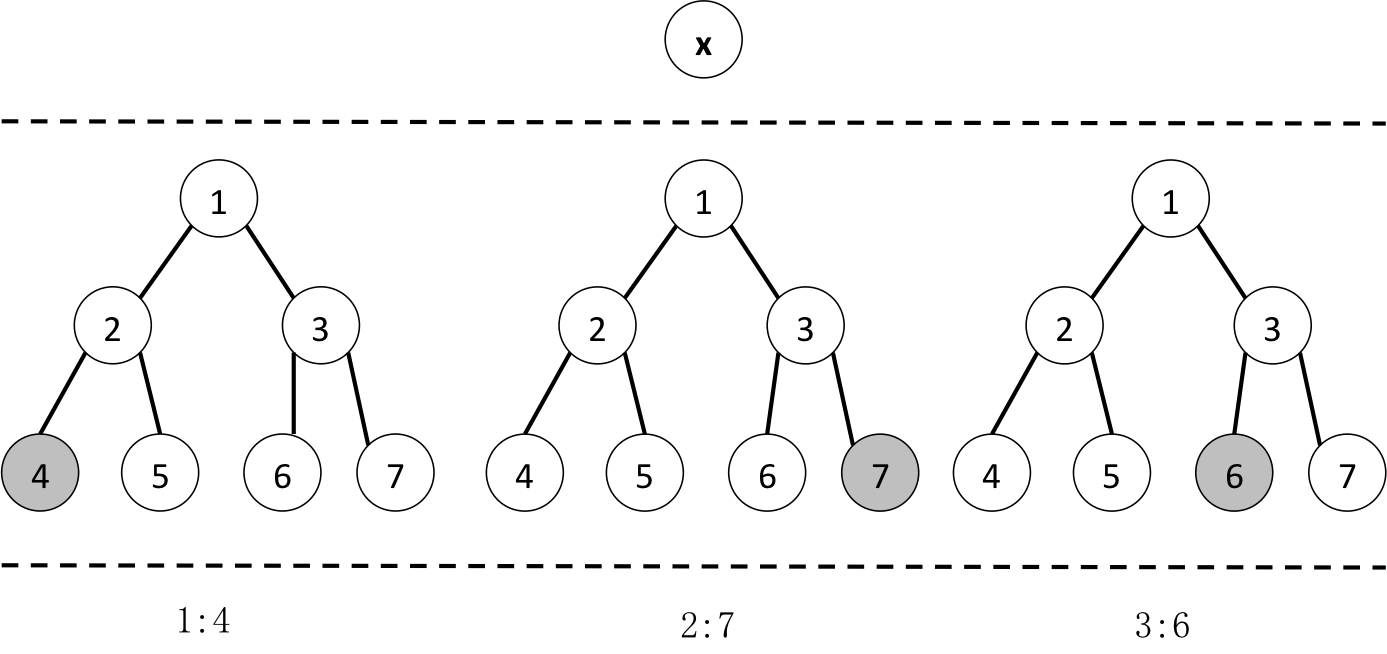
\includegraphics[width=0.8\textwidth]{GBDT.png}
\caption{The GBDT can be used to generate new features}
\label{fig:GBDT}
\end{figure}

The representational power of deep interaction-product network is usually applied to deep learning in speech recognition and computer vision. The dimension of feature is extremely high in computational advertisement if considering all feature interaction. Suppose we have $N$ single features, the candidate of combination of features will be $2^{N}$. The sparse learning algorithm cannot learn parameters properly. 

\begin{figure}[htbp]
\centering
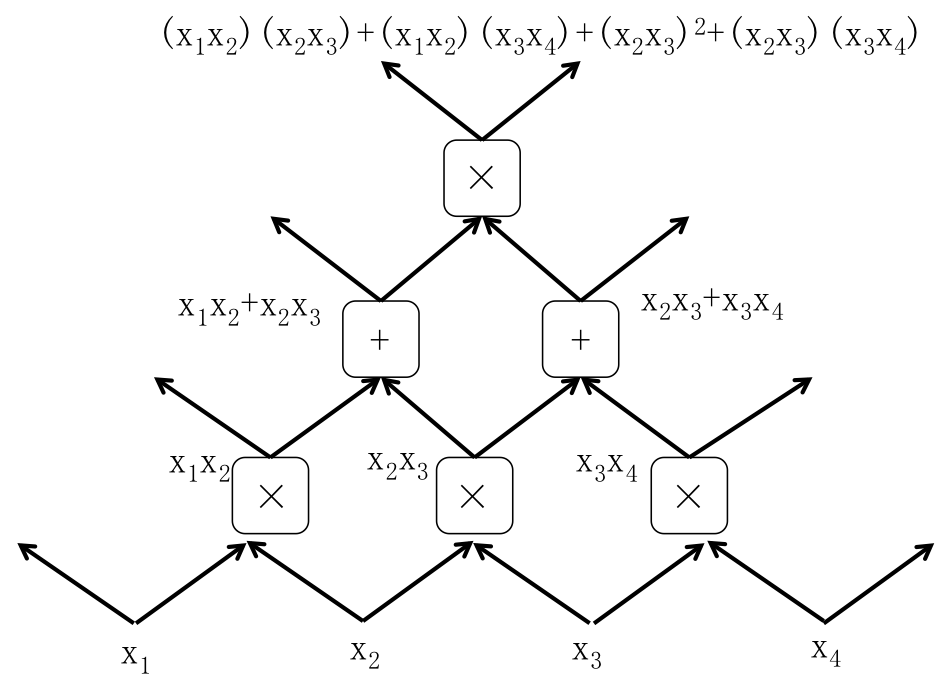
\includegraphics[width=0.7\textwidth]{DANOVA.png}
\caption{The deep structure of DANOVA for feature engineering}
\label{fig:DANOVA}
\end{figure}

As a deep structure, the method called DANOVA \cite{yoshuabengioolivierdelalleau2012,olivierdelalleauyoshuabengio2012} is well effective for feature engineering. It is a greedy combination starting from single features to stepwise feature interactions. The efficiency of feature mining will increase round hundreds times and save plenty of memory for computing. The basic idea is shown in Figure~\ref{fig:DANOVA}.


\begin{figure}[htbp]
\centering
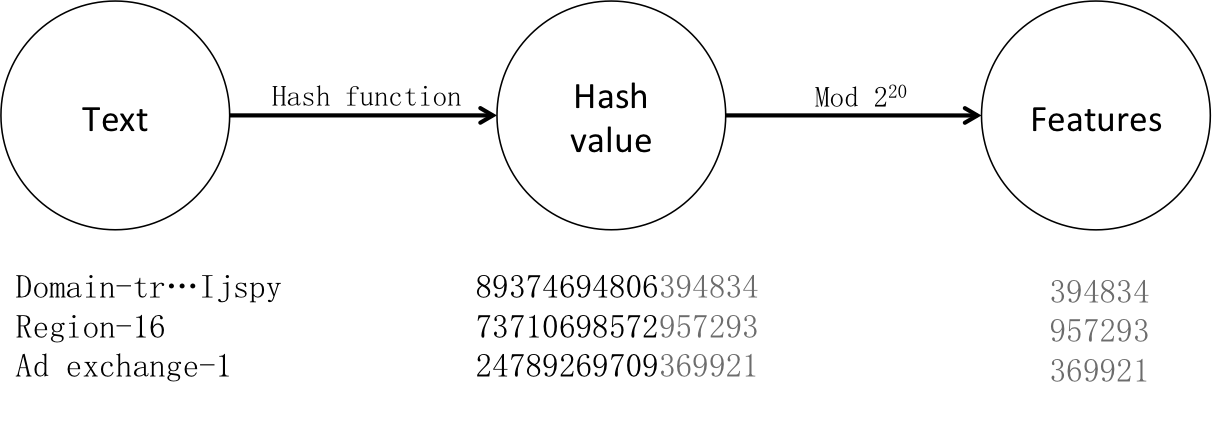
\includegraphics[width=0.8\textwidth]{hashing.png}
\caption{The hashing trick is used to save RAM for computation}
\label{fig:hashing}
\end{figure}

Categorical features appear less than 10 times are transformed into a special value. GBDT features and interaction features based on deep structure are directly included. These groups of features are hashed into $2^{20}$ dimension by hashing trick in Figure~\ref{fig:hashing}. 

Besides, there are some additional ways to generate features: Counting Features, Bag Features, Click History, etc.

\section{Online Learning Algorithms}

iPinYou dataset used in this project is about 16 GB. In terms of a single advertiser, the size of date is still around 2 GB. To the best of our knowledge, it is very difficult to learn model using the whole dataset or mini-batch as the memory in one machine is not enough. Online learning is designed for a sequential data stream. The predictive model is updated after receiving a new data point. It could be used in the case of a process occurring in time. 

The uncertain CTR as an important KPI faces a random distribution of competing bids in each auction. A few online methods can help to estimate its true value. FTRL-proximal online learning algorithm designed by Google is an excellent deterministic and parametric approach to solve large-scale sparsity and convergence issues, but it lacks the prediction of variance of the estimator \cite{h.brendanmcmahangaryholt2013}. Bayesian Online Probit Regression (BOPR) is from Microsoft Bing. It is an online probabilistic way to obtain estimated CTR. The distribution of estimator can be approximated by sampling and updating \cite{thoregraepeljoaquinquinonerocandelathomasborchertralfherbrich2010}. The paper written by Facebook team \cite{xinranhejunfengpanetc2014} gives a comparison between these two methods and also implies the feature engineering insight using Gradient Boosting Decision Trees (GBDT) that can improve the predicting performance. Besides, Field-aware Factorization Machine (FFM) which is widely used in collaborative filtering can provide a new form of estimator \cite{michaeljahrerandreastscherjeongyoonleejingjingdeng2012, steffenrendle2010}. It usually has outperformance than other linear estimator based methods.

\subsection{Bayesian Online Probit Regression (BOPR)}
In this section, we introduction a Bayesian CTR estimation algorithm. We build a generalized linear model with a probit link function to predict CTR. Before illustrating existing models, we introduce some basic notations in Table~\ref{tab:BOPR}:


\begin{table}[H]
\caption{Notation and description of BOPR}
\label{tab:BOPR}
\begin{center}
\begin{tabular}{ l l } 
\hline
Notation & Description \\
\hline
$\mathbf{x}$ & The bid request which is determined by its sparse and binary \\
& feature vector after one-hot encoding\\
$\mathbf{w}$ & The weight which is a linear estimator of probit link function\\
$y$ & Binary label of click \\
$\theta$ & Click-through rate \\
$\bm{\mu }$ & A vector of means of the weight \\
$\bm{\sigma }$ & A vector of variances of the weight \\
$\Sigma$ & Total variance of a given input \\
$s, t$ & Latent variables for factorization density function\\
$f$ & Sample weight from Gaussian prior\\
$g$ & The score $s$ for $\mathbf{x}$ as the inner product\\
$h$ & Factor to obtain $t$ from $s$ by adding zero-mean Gaussian noise \\
$q$ & Click value mapped by a threshold and Sigmoid function \\
\hline
\end{tabular}
\end{center}
\end {table}
After feature transformation, an ad feature becomes a binary encoding vector $\mathbf{x}=(\mathbf{x}_{j1},...,\mathbf{x}_{jk})$ where $\mathbf{x}_{j}$ is the $j$-th discrete feature for all $j\in\left \{ 1,...,J \right \}$ and $j1,...,jk$ are the values of the $k$ categories. We denote the total dimension of $\mathbf{x}$ is $d$. In order to arrive at Bayesian online learning for probit regression (BOPR), the likelihood and prior for advertiser $i$ are given by (we drop $i$ here)
\begin{equation}
\label{samplingprior}
p(y|\mathbf{x},\mathbf{w})=\Phi (\frac{y\cdot \mathbf{w}^{T} \mathbf{x}}{\beta })
\end{equation}
where $\Phi(t)$ is the cumulative density function of standard normal distribution and $N(t)$ is the density function of the standard normal distribution. The parameter $\beta$ scales the steepness of the inverse link function.
\begin{equation}
p(\mathbf{w})=\prod_{j=1}^{J} \prod_{k=1}^{K_j}N(w_{jk},\mu_{jk},\sigma_{jk}^2)
\end{equation}
In terms of the given sampling distribution Eq.~(\ref{samplingprior}), we can obtain the posterior probability of $\mathbf{w}$
\begin{equation}
p(\mathbf{w}|\mathbf{x},y) \propto p(y|\mathbf{x},\mathbf{w}) \cdot p(\mathbf{w})
\end{equation}
The distribution can be interpreted in Figure~\ref{fig:BOPR}.

\begin{figure}[htbp]
\centering

\includegraphics[width=0.5\textwidth]{BOPR.png}
\caption{Factor graph model of BOPR with message flow}
\label{fig:BOPR}
\end{figure}

We introduce two latent variables $t,s$ and three factors $f,g,h$ where $f$ is the sample weights $\mathbf{w}$ from the Gaussian prior, $s=\mathbf{w}^{T}\mathbf{x}$, $g$ gives $p(s|\mathbf{x},\mathbf{w})=\delta (s)$, $h$ adds zero-mean Gaussian noise to obtain $t$ from $s$ such that $p(t|s)=N(t;s,\beta^{2})$ and $q$ is a function such that $p(y|t)=\delta (y=sign (t))$. They satisfy a factorization relation
\begin{equation}
p(y,t,s,\mathbf{w}|t) \propto p(y|t) \cdot p(t|s) \cdot p(s|\mathbf{x},\mathbf{w}) \cdot p(\mathbf{w})
\end{equation}
In this application, the Bayesian online learning algorithm is based on the \emph{Stochastic Gradient Descent} (SGD) or \emph{Online Gradient Descent} (OGD), which attempts to update the posterior distribution of weight vector $\mathbf{w}$. The inference in the algorithm is to approximate $p(\mathbf{w}|y,\mathbf{x})$ and project it back to the closet factorizing Gaussian distribution of $p(\mathbf{w})$. The update equations for parameters $\bm{\mu }$ and $\bm{\sigma }$ are obtained as
\begin{equation}
\hat{\mu }_{{jk}}\leftarrow \mu _{{jk}}+yx_{{jk}}\cdot \frac{\sigma_{{jk}}^{2}}{\Sigma}\cdot \nu (\frac{y \cdot \mathbf{x}^{T}\bm{\mu}}{\Sigma })
\end{equation}
\begin{equation}
\hat{\sigma }^{2}_{{jk}}\leftarrow \sigma ^{2}_{{jk}}\cdot [1-x_{{jk}}\cdot \frac{\sigma_{{jk}}^{2}}{\Sigma ^{2}}\cdot q(\frac{y\cdot \mathbf{x}^{T}\bm{\mu }}{\Sigma })]
\end{equation}
\begin{equation}
\Sigma ^{2} := \beta ^{2}+\sum_{k=1}^{K_{j}}\sigma _{{jk}}^{2}
\end{equation}

\begin{figure}[htbp]
\centering
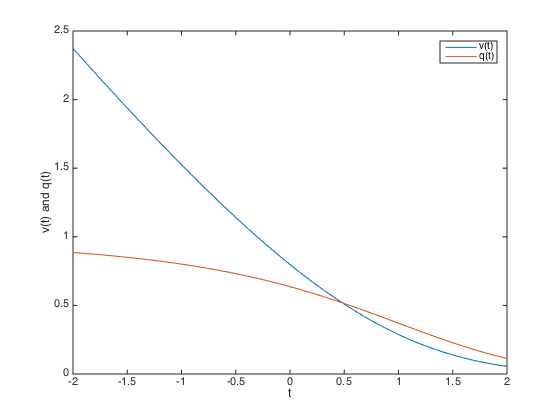
\includegraphics[width=0.8\textwidth]{vandq.png}
\caption{Plot of learning step size function $\nu(t)$ and $q(t)$}
\label{fig:vandq}
\end{figure}

The corrector functions $\nu$ and $q$ are given by $\nu(t):=N(t)/\Phi(t)$ and $q(t):=\nu (t)\cdot [\nu (t)+t]$ in Figure~\ref{fig:vandq}. In the regime $y \cdot \mathbf{x}^{T}\bm{\mu}<0$, the function $\nu(\cdot)$ grows almost linearly which plays a more significant role if errors happen. For the update equations, every observation will result in a decrease in variance of the weight. Therefore, the predictive function is the marginal distribution of the likelihood
\begin{equation}
p(y|\mathbf{x})=\int p(y|\mathbf{x},\mathbf{w})p(\mathbf{w})d\mathbf{w}=\Phi (\frac{y\cdot \mathbf{x}^{T}\bm{\mu}}{\Sigma })
\end{equation}
Comparing with the parameter defined and sampling distribution above, we have the inference result of CTR as
\begin{equation}
\theta=p(y=1|\mathbf{x})=\Phi (\frac{\mathbf{x}^{T}\bm{\mu}}{\Sigma })
\end{equation}
As the number of observation is large enough, the situation that variance converges to zero will occur. The prediction has some similarities as FTRL-Proximal which only considers the weight and ignores the change of variance. If variance is still needed, we can add some techniques like dynamics to generate a correction for variance.

\subsection{Follow the Regularized Leader (FTRL)}

As predicting CTR is a massive-scale learning problem, FTRL-Proximal online learning algorithm with good sparsity and convergence properties can be applied to exploring the dynamic system \cite{h.brendanmcmahan2011}. It will better the memory savings, visualizing performance, confidence estimation and calibration methods. We introduce some basic notations in Table~\ref{tab:FTRL}:
\begin{table}[H]
\caption{Notation and description of FTRL-Proximal}
\label{tab:FTRL}
\begin{center}
\begin{tabular}{ l l } 
\hline
Notation & Description \\
\hline
$\mathbf{x}$ & The bid request which is determined by its sparse and binary \\
& feature vector after one-hot encoding\\
$\mathbf{w}$ & The weight which is a linear estimator of logistic regression \\
$\mathbf{g}$ & The gradient of weight update \\
$y$ & Binary label of click \\
$\theta$ & Click-through rate \\
$t$ & The times of round \\
$\eta$ & A non-increasing learning rate \\
$\lambda$ & Regularization Parameter \\
\hline
\end{tabular}
\end{center}
\end {table}

To present how we can implement FTRL-Proximal precisely,  we also denote the compressed summation notation $\mathbf{g}_{1:t}=\sum_{s=1}^{t}\mathbf{g}_{s}$. We predict $\theta_t=\sigma(\mathbf{w}_t \cdot \mathbf{x}_t)$, where $\sigma(\cdot)$ is a sigmoid function. It can straightforward show the gradient at each round is given by $(\theta-y)\mathbf{x} \in \mathbb{R}^{d}$. However, SGD or OGD is not particularly effective for solving sparse models. To avoid this issue, \emph{Elastic Net} adds $L1$ regularization (known as Lasso) and $L2$ regularization (known as Ridge) to trade-off the degree of sparsity. By \emph{Following the Regularized Leader} (FTRL), the online gradient descent perform a update
\begin{equation}
\mathbf{w}_{t+1}=\mathbf{w}_{t}-\eta _{t} \cdot \mathbf{g}_{t}
\end{equation}

The learning rate is non-increasing. In order to be adaptive based on historical gradient, it is defined by
\begin{equation}
\eta _{t,i}=\frac{\alpha}{\beta + \sqrt{\sum_{s=1}^{t}g_{s,i}^{2}}}
\end{equation}
Hence, the FTRL-Proximal algorithm uses the update formulation given below
\begin{equation}
\label{FTRL}
\mathbf{w}_{t+1}=\underset{\mathbf{w}}\argmax (\mathbf{g}_{1:t} \cdot \mathbf{w} + \frac{1}{2}\sum_{s=1}^{t}\sigma_{s}\left \|\mathbf{w}-\mathbf{w}_s  \right \|_{2}^{2}+\lambda_{1}\left \|\mathbf{w}  \right \|_{1})
\end{equation}
where $\sigma_{1:t}=\frac{1}{\eta _{t}}$. This update seems to require storing all the past coefficients. It will lead to lower time sensitivity and looks much more complicated than common gradient descent. However, the memory can be saved indeed because we only need to store only one number per coefficient. The Eq.~(\ref{FTRL}) is rewritten as the argmin over $\mathbf{w} \in \mathbb{R}^{d}$ of
\begin{equation}
(\mathbf{g}_{1:t}-\sum_{s=1}^{t}\eta _{t}\mathbf{w}_{s})\cdot \mathbf{w}+\frac{1}{\eta _{t}}\left \|\mathbf{w} \right \|_{2}^{2}+ \lambda _{1} \left \|\mathbf{w}  \right \|_{1}+(const)
\end{equation}

Thus, if we store $\mathbf{z}_{t-1}=\mathbf{g}_{1:t-1}-\sum_{s=1}^{t-1}\sigma_{s}\mathbf{w}_{s}$ at the beginning of round $t$, we can add an intermediate substitution expressed by $\mathbf{z}_{t}$. The update lets
\begin{equation}
\mathbf{z}_{t}=\mathbf{z}_{t-1}+\mathbf{g}_{t}+(\frac{1}{\eta_t}-\frac{1}{\eta_{t-1}})\mathbf{w}_{t}
\end{equation}
and solve for $\mathbf{w}_{t+1}$ in closed form on a per-coordinate bases by
\begin{equation}
w_{t+1,i}=\left\{\begin{matrix}
0 &\mathrm{if } |z_{t,i}| \leq \lambda_{1} \\ 
 -\eta_t(z_{t,i}-sign(z_{t,i})\lambda_1) & \mathrm{otherwise}
\end{matrix}\right.
\end{equation}
It implies that only $\mathbf{z}_t$ needs to be stored in memory and we do not need to store the historical gradient since we can use $\mathbf{z}_t$ to show the previous situations. When $\lambda_1=0$, it transforms to be 
\begin{equation}
\mathbf{w}_{t+1} = -\eta_t \mathbf{z}_{t}=-\eta_t \sum_{s=1}^{t}\mathbf{g}_s
\end{equation}
In this case, the memory cost is exactly same as the normal gradient descent coefficient. Nevertheless, there is no free lunch. Even though FTRL-Proximal can deal with large-scale sparsity properly, it still has shortcomings comparing with BOPR. It is too complicated to generate a variance for the estimator because it is a deterministic approach.

\subsection{Field-aware Factorization Machine (FFM)}
The idea of FFM is firstly used in \emph{Collaborative Filtering} (CF) since the data table consisting of both fields and features. A technique called \emph{Alternative Least Squares} (ALS) is very applicable for the decomposition of association matrix and learning of latent factors. Estimation of CTR also can be treated as a FFM problem. We introduce some basic notations in Table.~\ref{tab:FFM}:
\begin{table}[H]
\caption{Notation and description of FFM}
\label{tab:FFM}
\begin{center}
\begin{tabular}{ l l } 
\hline
Notation & Description \\
\hline
$\mathbf{x}$ & The bid request which is a numerical feature vector\\
$\mathbf{w}$ & The weight which is a field  estimator \\
$\phi$ & The mapping function \\
$y$ & Binary label of click \\
$\theta$ & Click-through rate \\
\hline
\end{tabular}
\end{center}
\end {table}

The commonly applied mapping approaches for regression are like first order Linear Model and Degree-2 Polynomial Model . The feature mapping functions like those in \emph{Support Vector Machine} (SVM) are given by
\begin{itemize}
  \item Linear Model:
	\begin{equation}
	\phi (\mathbf{w},\mathbf{x})=\sum_{j \in C}w_{j}x_{j}
	\end{equation}
  \item Degree-2 Polynomial Model (Ploy2):
	\begin{equation}
	\phi (\mathbf{w},\mathbf{x})=\sum_{j_1,j_2 \in C}{w}_{j_1, j_2}x_{j_1}x_{j_2}
	\end{equation}
\end{itemize}
In the above situations, the weight as coefficient is a scalar value for the single feature vector or the interaction of different feature vectors.  However, based on the well known regression models, for \emph{Factorization Machine} (FM) \cite{michaeljahrerandreastscherjeongyoonleejingjingdeng2012}, the form is more extensive. The current coefficient is the inner product of weight vectors. The weight vector $\mathbf{w} \in \mathbb{R}^{d} $ is a latent factor used to describe the fields and features. The mathematical formulations for FM and FFM \cite{steffenrendlelarsschmidtthieme2010} are
\begin{itemize}
	\item Factorization Machines (FM):
		\begin{equation}
		\phi (\mathbf{w},\mathbf{x})=\sum_{j_1,j_2 \in C}<\mathbf{w}_{j_1},\mathbf{w}_{j_2}>x_{j_1}x_{j_2}
		\end{equation}
	\item Field-aware Factorization Machines (FFM):
		\begin{equation}
		\phi (\mathbf{w},\mathbf{x})=\sum_{j_1,j_2 \in C}<\mathbf{w}_{j_1,f_2},\mathbf{w}_{j_2,f_1}>x_{j_1}x_{j_2}
		\end{equation}		
\end{itemize}

Let us show a concrete FFM example of overall CTR estimation in practice, which only includes three advertiser fields and five ad features. We want to map categorical values into corresponding field indexes and feature indexes. The mapping relationship is in Table~\ref{tab:FFMCTR}.

\begin{table}[H]
\caption{A concrete FFM example of overall CTR estimation in practice}
\label{tab:FFMCTR}
\begin{tabular}{ p{3cm}p{3cm}|p{3cm}p{3cm}  }
 \hline
 \multicolumn{4}{c}{Fields and Features Mapping} \\
 \hline
Field Name & Field Index & Feature Name & Feature Index \\
 \hline
Ader ID-1458  & field \color{red}{1}    & UserAgent-window-chrome &  feature \color{blue}{5}\\
Ader ID-2259 & field \color{red}{2}  & City-11  & feature \color{blue}{8}\\
AderID-2261 & field \color{red}{3} & Ad slot format-1 & feature \color{blue}{17}\\
 & & Region-16 & feature \color{blue}{5} \\
  & & UserTags-10006 & feature \color{blue}{6} \\
 \hline
\end{tabular}
\end{table}

After transformation to the FFM format, the encoding of data raises as 
\begin{center}
\color{red}{1}:\color{blue}{5}:\color{black}{1}	\color{red}{2}:\color{blue}{8}:\color{black}{0}	\color{red}{3}:\color{blue}{17}:\color{black}{1}	\color{red}{2}:\color{blue}{5}:\color{black}{1}	\color{red}{1}:\color{blue}{6}:\color{black}{1}
\end{center}
For FFM, $\phi (\mathbf{w},\mathbf{x})$ is
\begin{equation}
\begin{split}
& <\mathbf{w}_{\color{red}{1},\color{blue}{5}}, \mathbf{w}_{\color{red}{2},\color{blue}{8}}> \cdot {1} \cdot 0 + <\mathbf{w}_{\color{red}{1},\color{blue}{5}}, \mathbf{w}_{\color{red}{3},\color{blue}{17}}> \cdot 1 \cdot 1 + <\mathbf{w}_{\color{red}{1},\color{blue}{5}}, \mathbf{w}_{\color{red}{2},\color{blue}{5}}> \cdot 1 \cdot 1 + <\mathbf{w}_{\color{red}{1},\color{blue}{5}}, \mathbf{w}_{\color{red}{1},\color{blue}{6}}> \cdot 1 \cdot 1 \\
& <\mathbf{w}_{\color{red}{2},\color{blue}{8}}, \mathbf{w}_{\color{red}{3},\color{blue}{17}}> \cdot 0 \cdot 1 + <\mathbf{w}_{\color{red}{2},\color{blue}{8}}, \mathbf{w}_{\color{red}{2},\color{blue}{5}}> \cdot 0 \cdot 1 + <\mathbf{w}_{\color{red}{2},\color{blue}{8}}, \mathbf{w}_{\color{red}{1},\color{blue}{6}}> \cdot 0 \cdot 1 \\
& <\mathbf{w}_{\color{red}{3},\color{blue}{17}}, \mathbf{w}_{\color{red}{2},\color{blue}{5}}> \cdot 1 \cdot 1 + <\mathbf{w}_{\color{red}{3},\color{blue}{17}}, \mathbf{w}_{\color{red}{1},\color{blue}{6}}> \cdot 1 \cdot 1 \\
& <\mathbf{w}_{\color{red}{2},\color{blue}{5}}, \mathbf{w}_{\color{red}{1},\color{blue}{6}}> \cdot 1 \cdot 1
\end{split}
\end{equation}
Unlike nonlinear SVMs, a transformation in the dual form is not necessary and the model parameters of FFM can be estimated directly without the need of any support vector. Also, FFM has the advantages in sparse settings \cite{steffenrendle2010}. Besides feature interactions, first order features are also used in FFM model. Thus, the optimization problem is
\begin{equation}
\underset{\mathbf{w}}{\min}\frac{1}{L} \sum_{i=1}^{L}(\log (1+\exp (-y_i \phi (\mathbf{w}, \mathbf{x}_i)))+\frac{\lambda}{2}\left \| \mathbf{w} \right \|^{2})
\end{equation}
where 
\begin{equation}
\phi (\mathbf{w},\mathbf{x})=\sum_{j_1,j_2 \in C}<\mathbf{w}_{j_1,f_2},\mathbf{w}_{j_2,f_1}>x_{j_1}x_{j_2}+\sum_{j \in C}w_{j}x_{j}
\end{equation}
The results of FM and FFM are identical or very similar to many of the specialized state-of-the-art models.










